\section{Results}

\begin{frame}
\frametitle{Overview of results}
\begin{enumerate}
\item Results for tridiagonal solver (NEATO)
\begin{itemize}
    \item Global memory v/s shared memory implementations
    \item Compared with library solvers
        (multicore CPU and GPU)
\end{itemize}
\item Results for compact finite difference application
\begin{itemize}
    \item Profiling results
    \item Scaling results
    \item Comparison with CPU-only approach
\end{itemize}
\end{enumerate}
\end{frame}

\begin{frame}
\frametitle{Global memory v/s shared memory implementations}
\footnotesize
\begin{columns}
\begin{column}{0.5\textwidth}

\begin{block}{Benchmark details}
\begin{itemize}
\item Solving multiple tridiagonal systems on single GPU
\item Up to $2048$ systems with $2048$ equations (2-D)
    and $512^2$ systems with $512$ equations (3-D)
\item GPU: NVIDIA Tesla K20
\end{itemize}
\end{block}

\begin{itemize}
\item For 2-D problems, shared memory clearly better
\item For 3-D problems, shared memory speedup
    is smaller
\item \textbf{Thread inactivity} in shared memory leads
    to reduced performance
\end{itemize}
\end{column}
\begin{column}{0.5\textwidth}
\centering
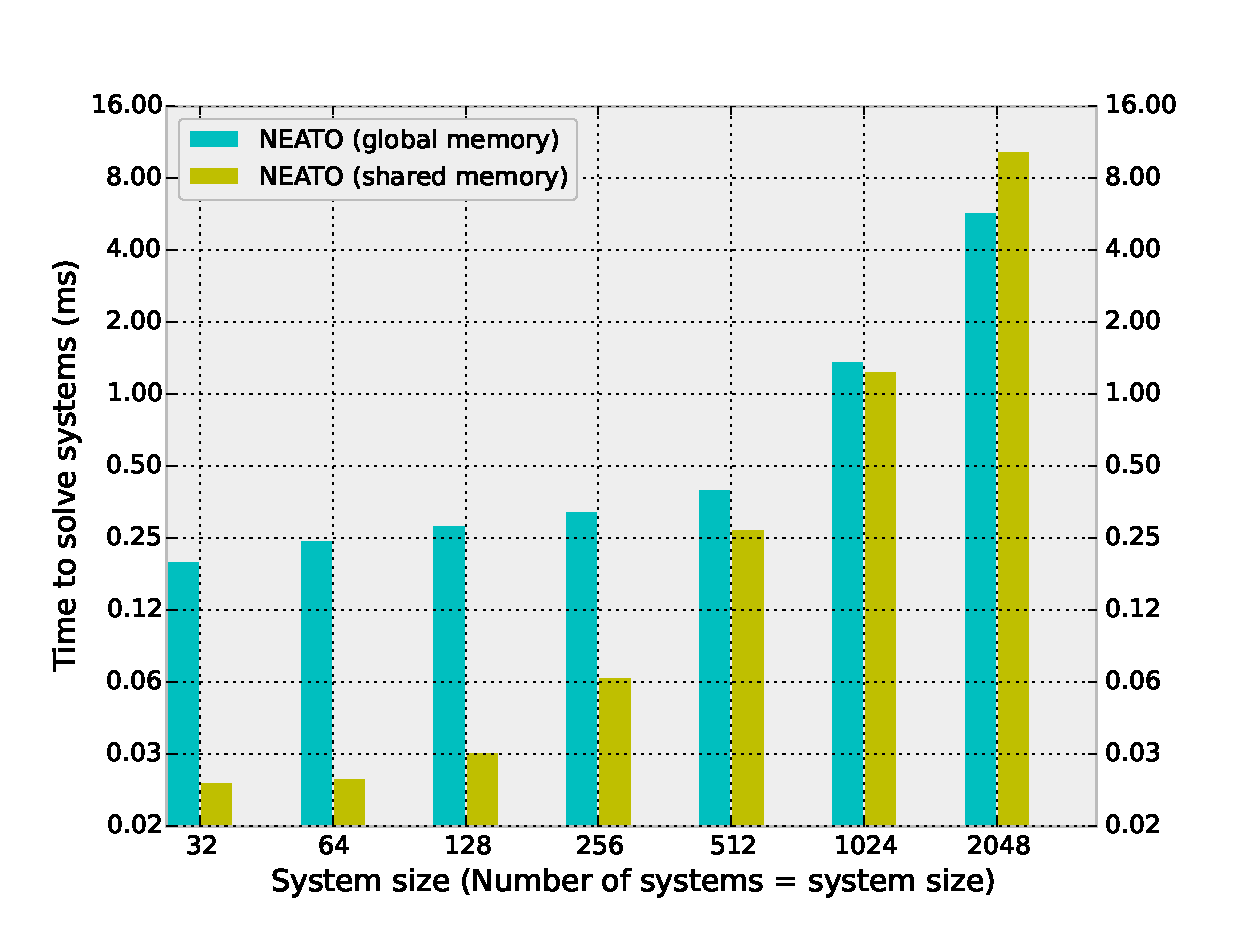
\includegraphics[width=140px]{img/global-vs-shared-2d.eps}

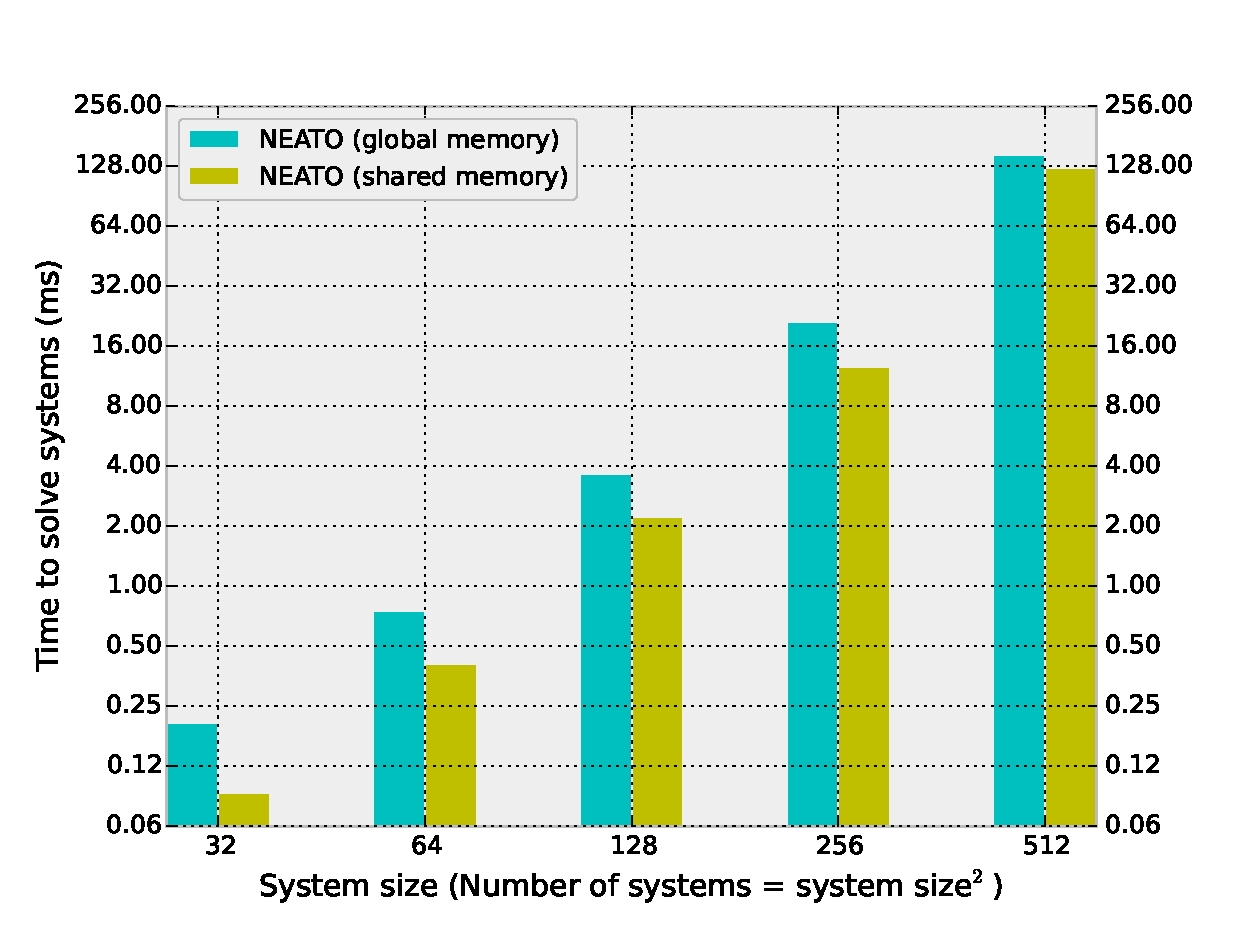
\includegraphics[width=140px]{img/global-vs-shared-3d.eps}
\end{column}
\end{columns}
\end{frame}

\begin{frame}{Comparison with library solvers}
\footnotesize
\begin{block}{Benchmark details}
\begin{itemize}
\item Solving multiple tridiagonal systems on single GPU and multicore CPU
\item Up to $2048$ equations in $2048$ variables (2-D)
    and $512^2$ equations in $512$ variables (3-D)
\item GPU: NVIDIA Tesla K20
\item CPU: Intel Xeon E5 v2
\item Do \emph{not} include cost of CPU-GPU transfer
\item Library solver details:
\begin{itemize}
    \footnotesize
    \item Intel MKL \texttt{dgtsv} (Gaussian elimination with partial pivoting)
    \item CUSPARSE \texttt{dgtsv} (Hybrid CR+PCR)
\end{itemize}
\item \texttt{-02} level compiler optimizations
\item Double precision
\item Comparison with up to 16 CPU cores
\end{itemize}
\end{block}
\end{frame}

\begin{frame}
\frametitle{Comparison with library solvers - speedup}
Speedups over library implementations:

\begin{figure}
\begin{minipage}{.45\textwidth}
    \centering
    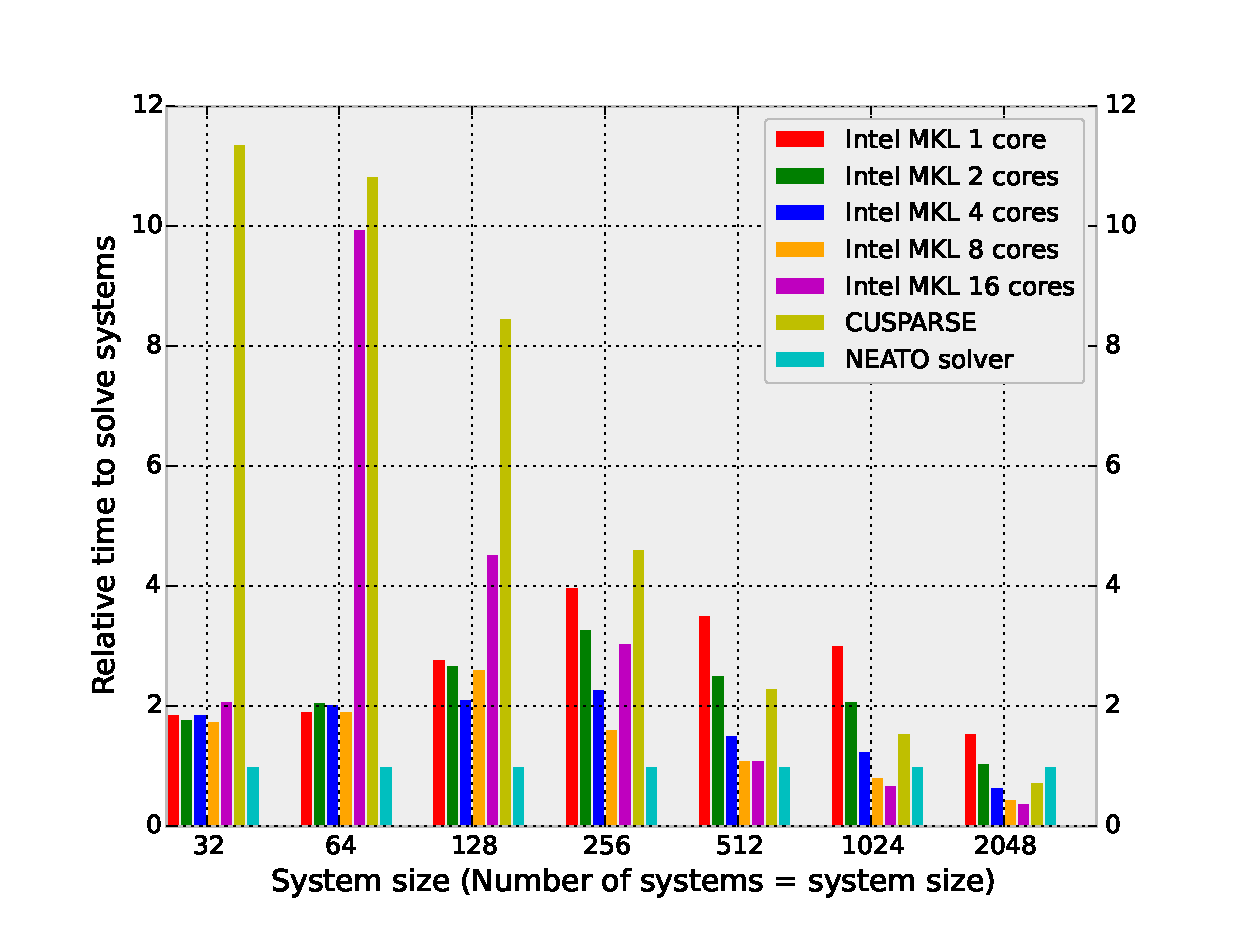
\includegraphics[width=\linewidth]{img/bench-2d.eps}
    \caption{2-D problems}
\end{minipage}
\begin{minipage}{.45\textwidth}
    \centering
    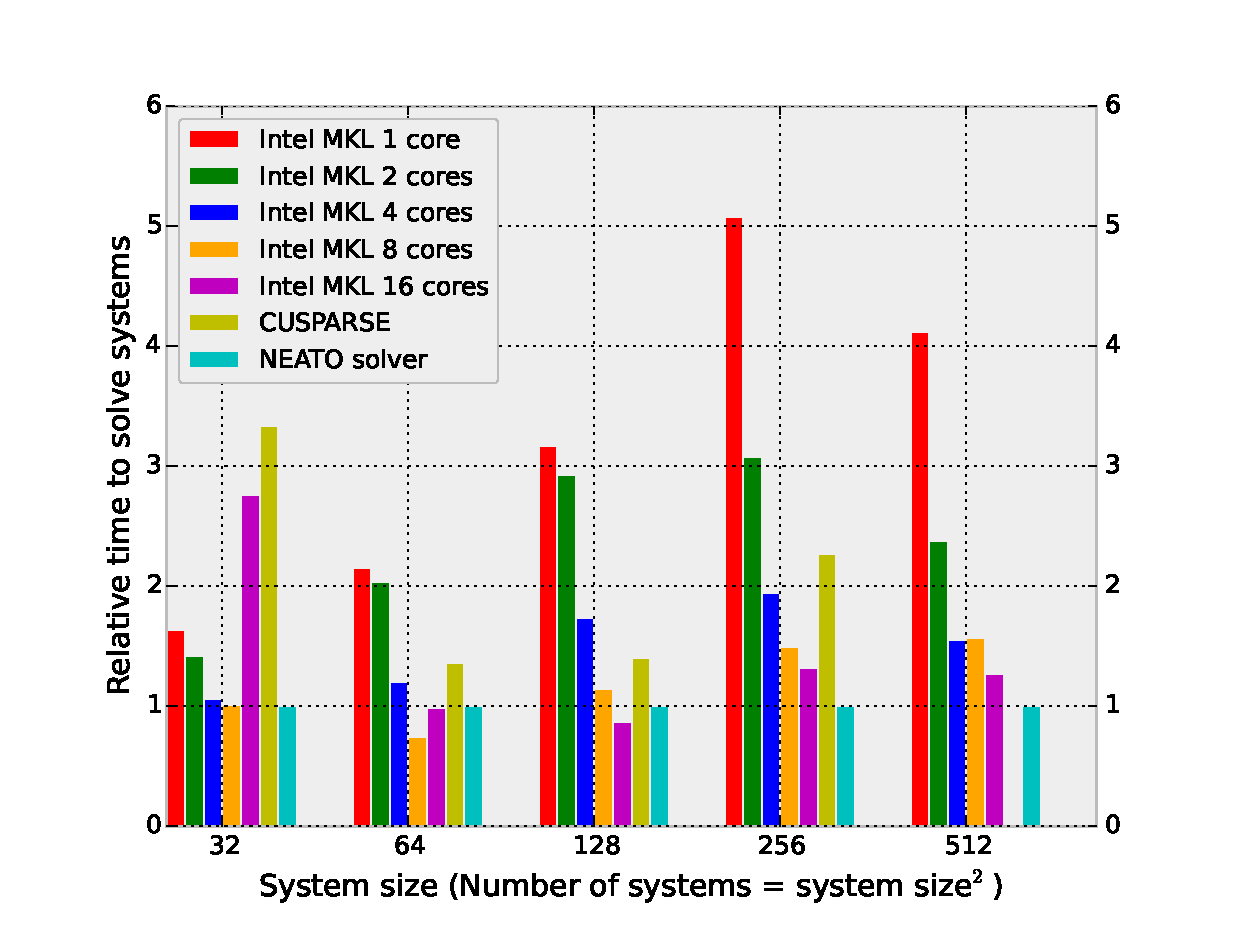
\includegraphics[width=\linewidth]{img/bench-3d.eps}
    \caption{3-D problems}
\end{minipage}
\end{figure}
\end{frame}

\begin{frame}
\frametitle{Notes on speedups}
\begin{itemize}
 
\item Faster than CUSPARSE in almost all cases
\begin{itemize}
    \item Can accomodate larger problems than CUSPARSE
\end{itemize}
\item Multicore CPU performance flattens out
\item Compared with 8 CPU cores, speedups over MKL in the range 1-2x
\item Solving the tridiagonal systems
    \emph{least amenable to efficient parallel solution}
\item Primary objective is to keep the problem on the GPU
\end{itemize}
\end{frame}

\begin{frame}{Compact finite difference evaluation}
\begin{block}{Benchmark details}
\begin{itemize}
\item Compact finite difference evaluation in 3-D for a function $f(x, y, z)$
\item Problem size up to $2048^3$ on up to 64 GPUs and 512 CPU cores
\item Tests performed on Palmetto cluster (Infiniband interconnect)
\end{itemize}
\end{block}
\end{frame}

\begin{frame}
\frametitle{Compact finite difference evaluation - profiling}
\begin{columns}
\begin{column}{0.5\textwidth}
\begin{itemize}
\item Most time spent on solving tridiagonal systems
    \begin{itemize}
        \item Justifies optimization effort
    \end{itemize}
\item Compute/communicate ratio increases with
    problem size
\item Significant portion of time spent on
    data permutation
    \begin{itemize}
        \item na\"{\i}ve implementation
    \end{itemize}
\end{itemize}
\end{column}
\begin{column}{0.5\textwidth}
\centering
\begin{figure}
\centering
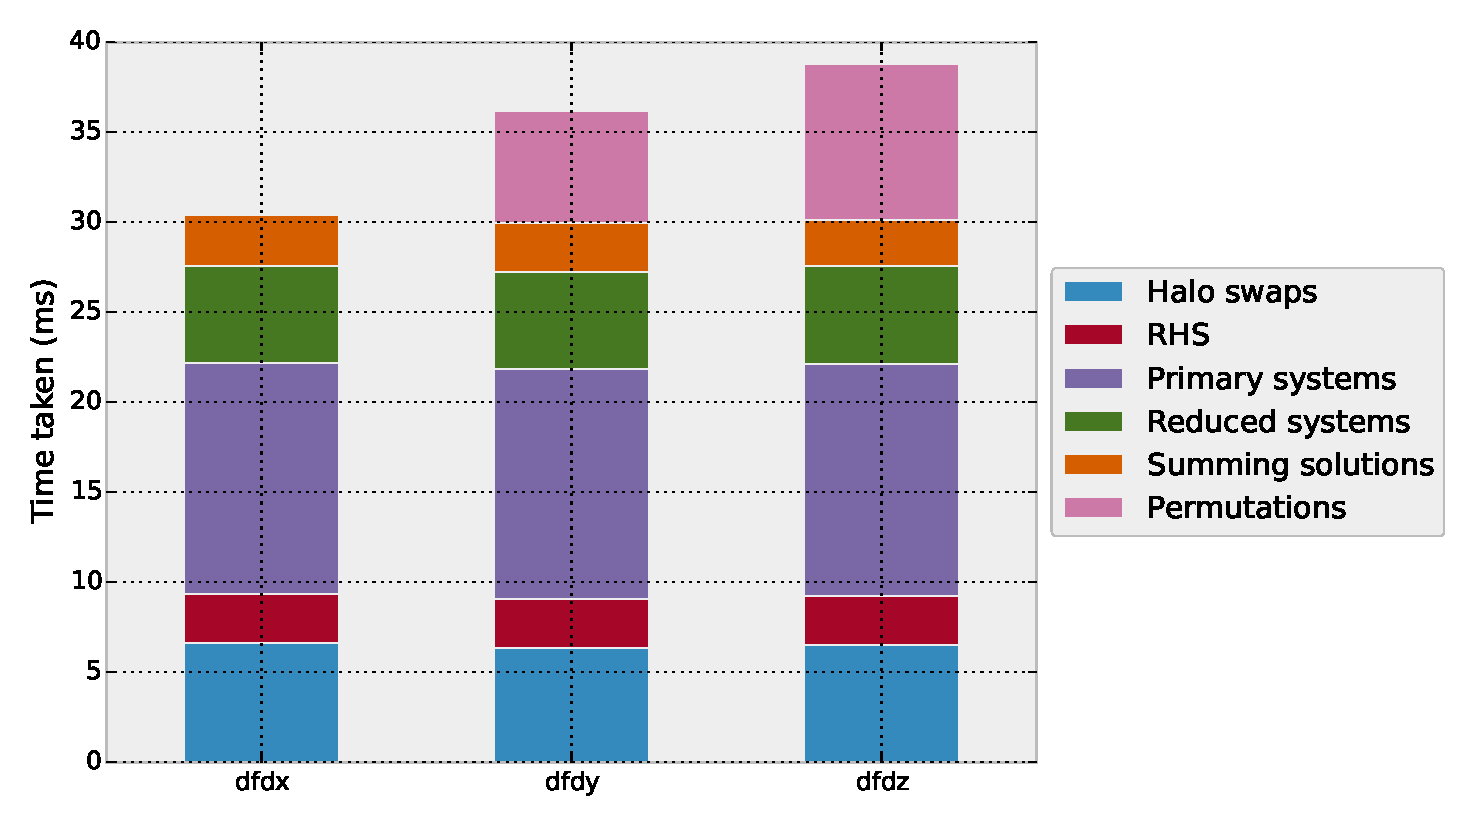
\includegraphics[width=150px]{img/profiling-1024-64.eps}

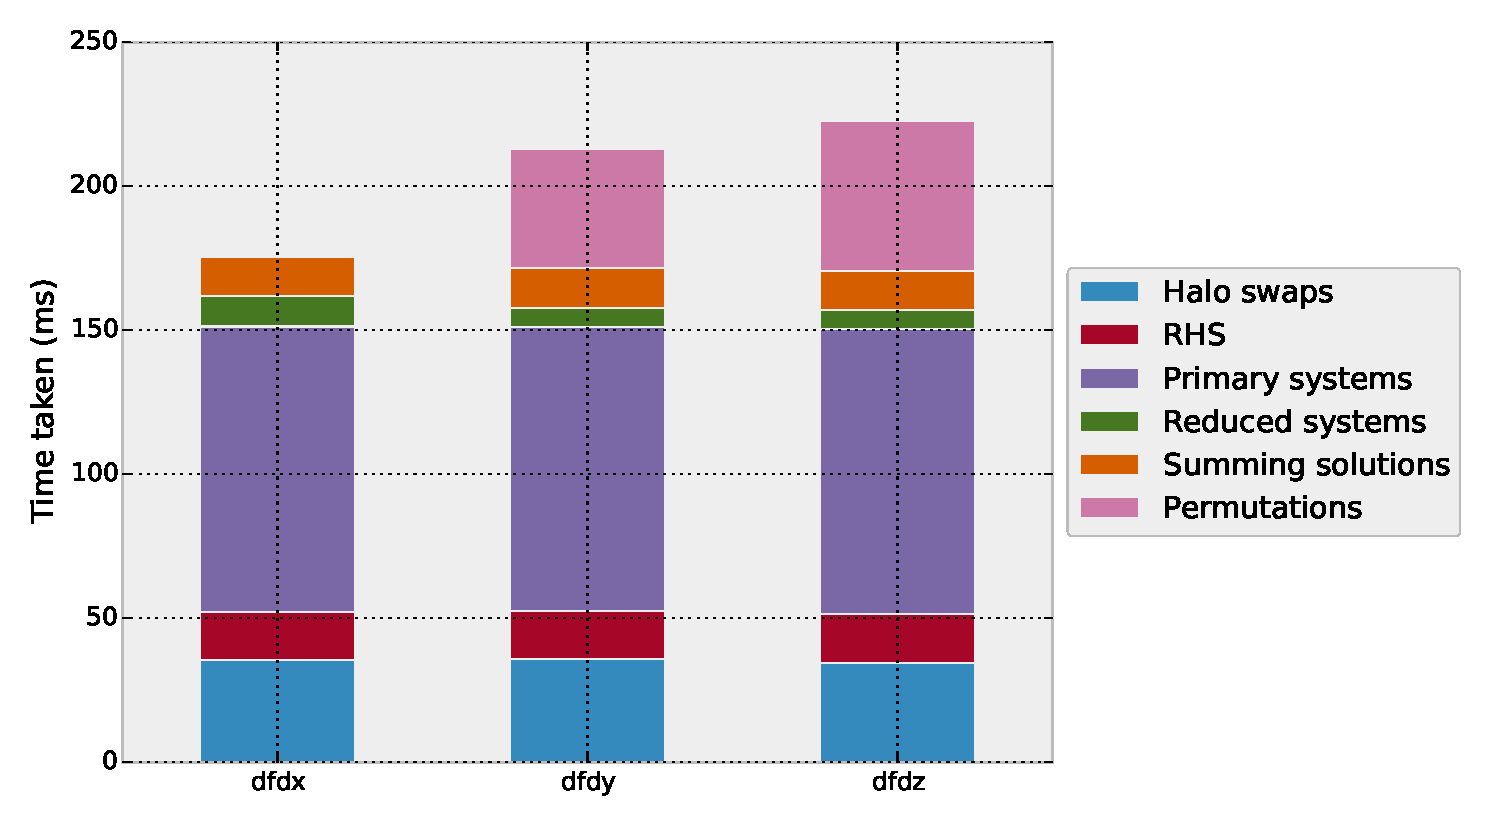
\includegraphics[width=150px]{img/profiling-2048-64.eps}
\caption{Problem sizes: $1024^3$ (above)
    and $2048^3$ (below) - 64 GPUs}
\end{figure}
\end{column}
\end{columns}
\end{frame}

\begin{frame}
\frametitle{Compact finite difference evaluation - strong scaling}
\begin{figure}
\begin{minipage}{.45\textwidth}
\centering
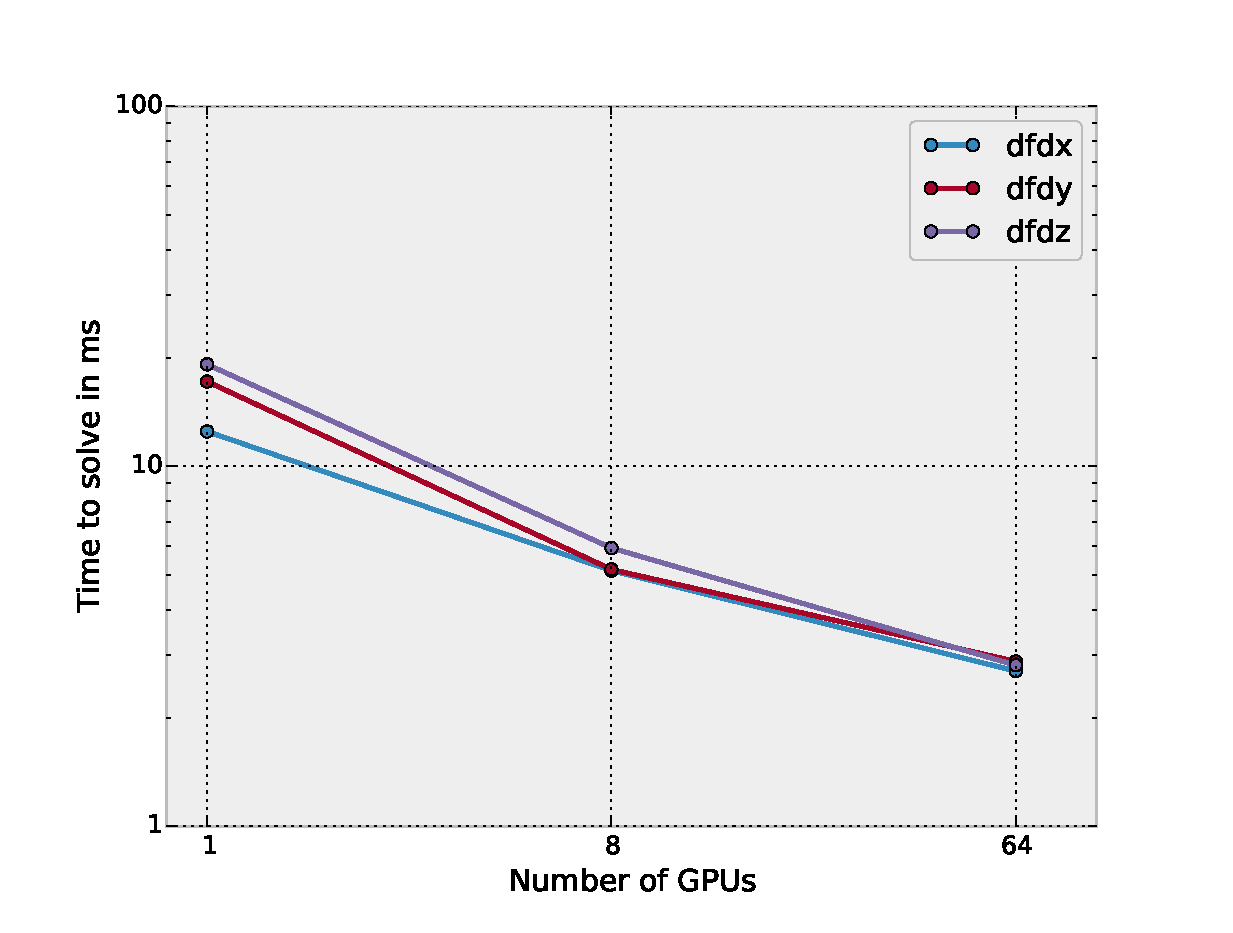
\includegraphics[width=\linewidth]{img/strong-scaling-256.eps}
\caption{Problem size: $256^3$}
\end{minipage}
\begin{minipage}{.45\textwidth}
\centering
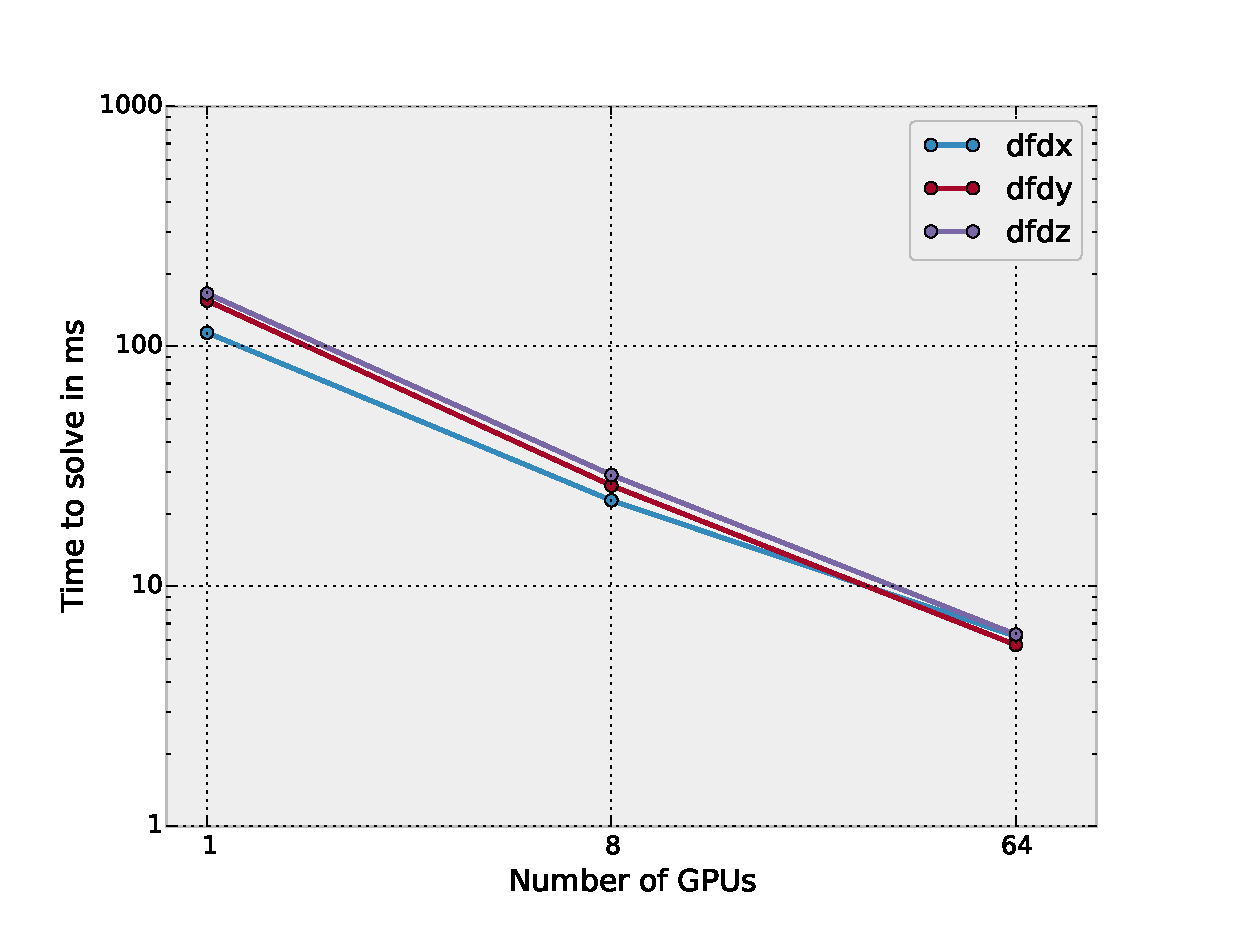
\includegraphics[width=\linewidth]{img/strong-scaling-512.eps}
\caption{Problem size: $512^3$}
\end{minipage}
\end{figure}
\centering
\end{frame}

\begin{frame}
\frametitle{Compact finite difference evaluation - strong scaling}
\begin{figure}
\begin{minipage}{.45\textwidth}
\centering
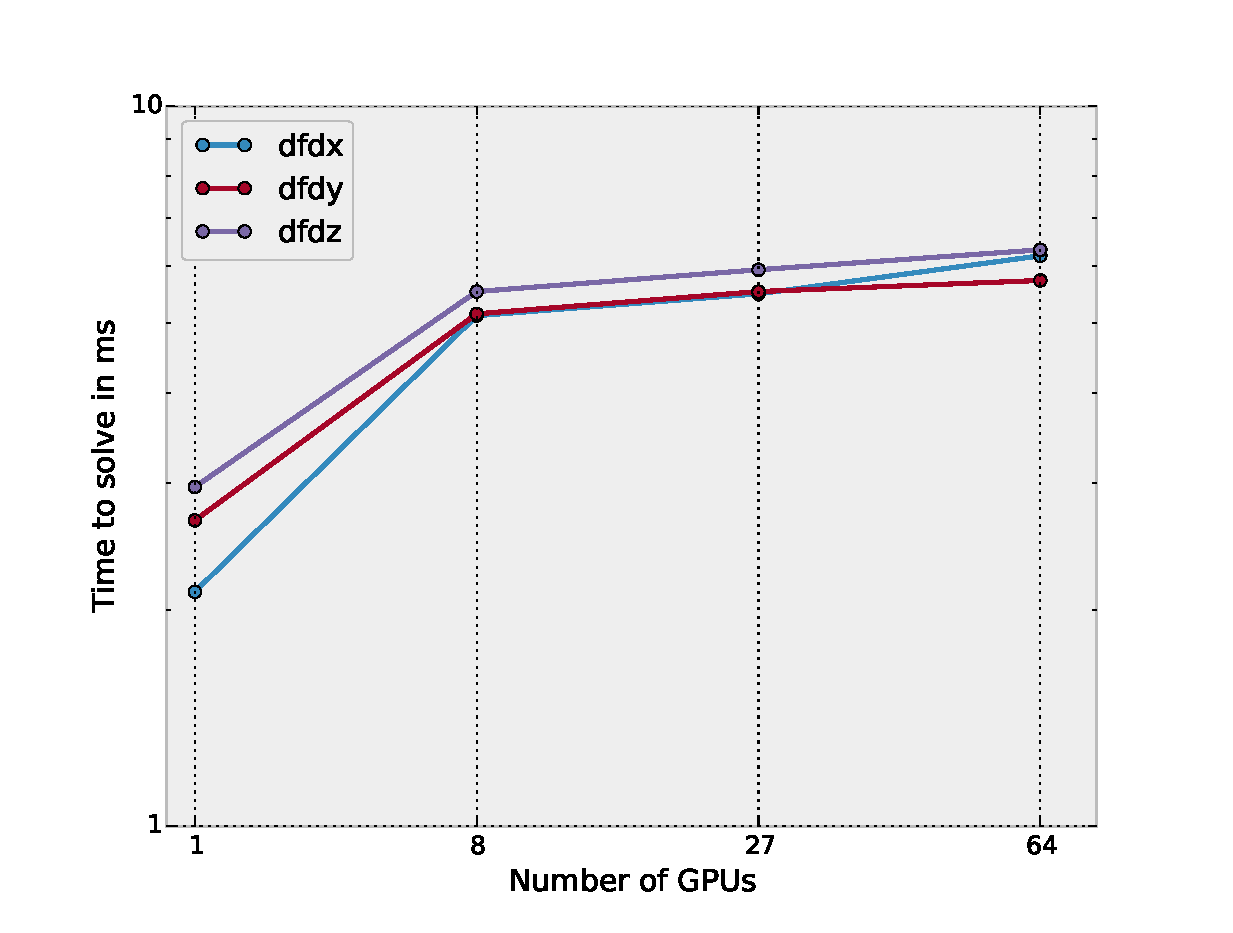
\includegraphics[width=\linewidth]{img/weak-scaling-128.eps}
\caption{Problem size \emph{per GPU}: $128^3$}
\end{minipage}
\begin{minipage}{.45\textwidth}
\centering
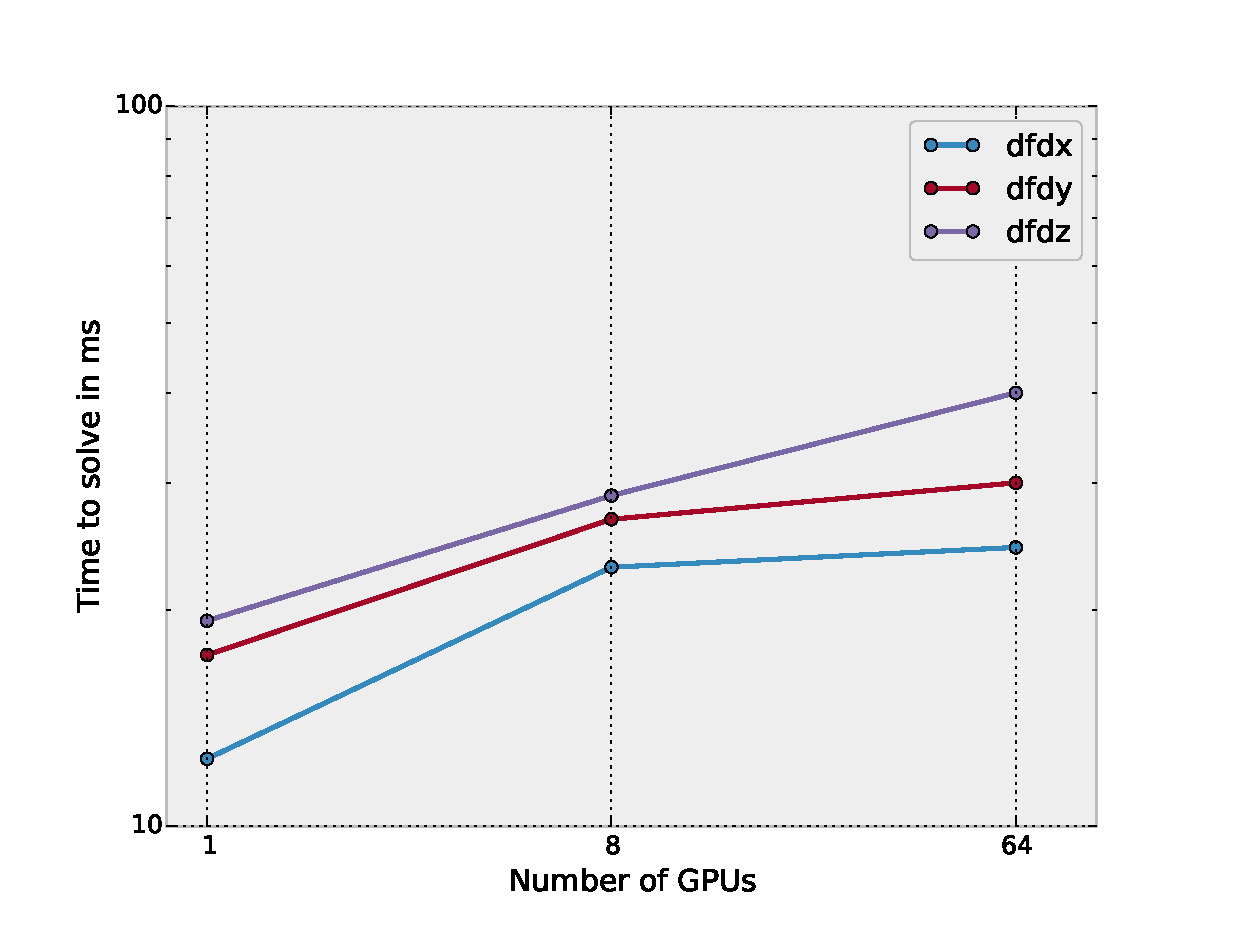
\includegraphics[width=\linewidth]{img/weak-scaling-256.eps}
\caption{Problem size \emph{per GPU}: $256^3$}
\end{minipage}
\end{figure}
\centering
\end{frame}

\begin{frame}
\frametitle{Comparison with CPU-only approach}
\begin{columns}
\begin{column}{0.5\textwidth}
\begin{itemize}
\item Reference implementation: CFDNS
    (Los Alamos National Lab)
\item Uses LU algorithm
\item Parallelized among individual cores
\item Maintain a ratio of 8 CPU cores : 1 GPU for comparison
\item Speedups  in the range 3-9x
\item NEATO has strong potential for GPU-based clusters
\end{itemize}
\end{column}
\begin{column}{0.5\textwidth}
\centering
\begin{table}
\resizebox{0.75\textwidth}{!}{%
\centering
\begin{tabular}{|l|l|l|l|l|l|l|}
\hline
\multirow{2}{*}{Size} & \multicolumn{3}{c|}{Ref. impl, \#CPU cores} & \multicolumn{3}{c|}{NEATO-based, \#GPUs} \\ \cline{2-7}
         & 8         & 64        & 512      & 1       & 8       & 64      \\ \hline
$256^3$  & 79.5      & 20.8      & 11.1     & 19.9    & 5.17    & 2.79    \\ \hline
$512^3$  & 556.8     & 146.5     & 29.2     & 164.5   & 23.24   & 5.62    \\ \hline
$1024^3$ & 5188      & 1092      & 223.7    & -       & 174.9   & 24.49   \\ \hline
$2048^3$ & -         & -         & 1741     & -       & -       & 297.07  \\ \hline
\end{tabular}

}
\end{table}

\includegraphics[width=160px]{img/compact-refimpl-speedups.eps}
\end{column}
\end{columns}
\end{frame}

\begin{frame}
\frametitle{Conclusions and future work}
\begin{itemize}
    \item Tridiagonal solver performance
        is key in compact finite difference evaluation
    \item Simple matrix structure can be exploited
        in the cyclic reduction algorithm
    \item Substantial speedups can be achieved
        over CPU
    \item Applicability to other algorithms: PCR, CR+PCR
    \item Integration into current DNS code
    \item Strategies for MIC architecures
\end{itemize}
\end{frame}

\begin{frame}
    Thank you    
\end{frame}

